\section{Diagrammes de cas d'utilisation}
	\label{sec:cas_utilisation}

	Lorsque l'utilisateur (ou joueur) lancera le jeu, plusieurs choix s'offriront à lui. Les diagrammes de cas d'utilisation sont les plus adaptés pour illustrer les différentes possibilité.

	\subsection{Menu principal}
		Au lancement du jeu, le joueur se trouvera face au menu principal, qui lui permettra de lancer une partie avec ses réglages favoris.
		Les différentes possiblités sont illustrées Figure \ref{fig:cas_util_menu}.

		\begin{figure}[h!]
			\centering
			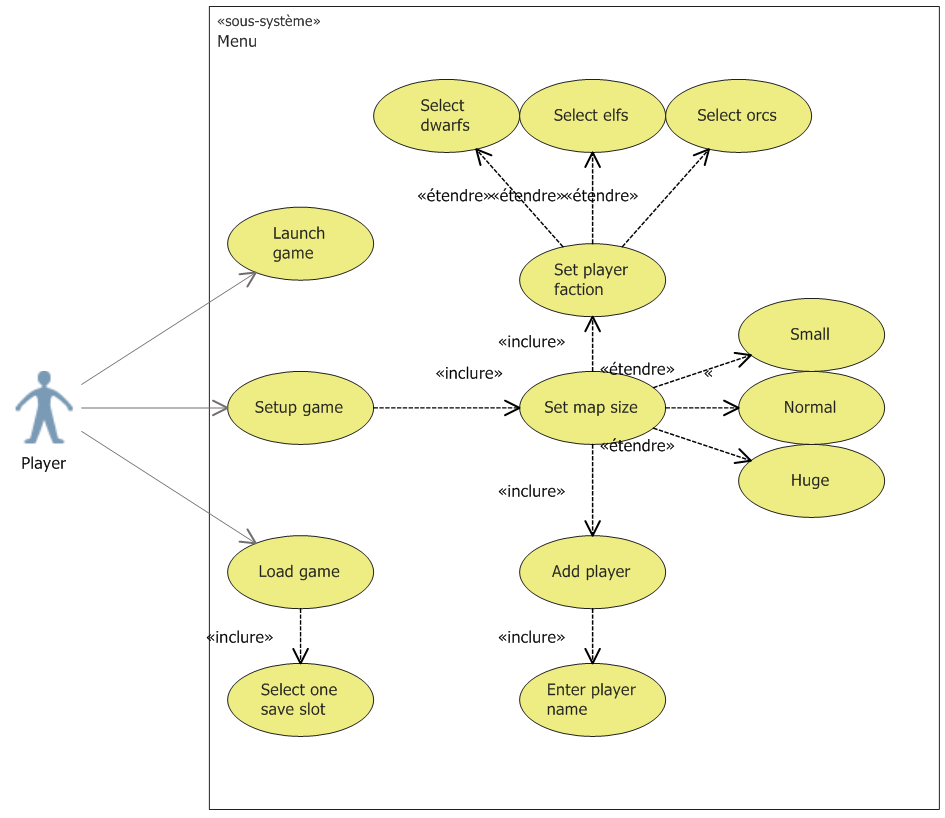
\includegraphics[width=1\textwidth]{figure/cas_util_menu.png}
			\caption{Diagramme de cas d'utilisation - Menu principal}
			\label{fig:cas_util_menu}
		\end{figure}

	\subsection{En cours de partie}
		Une partie pouvant avoir entre 2 et n joueurs, le diagramme de la Figure \ref{fig:cas_util_partie} illustre les différentes actions offertes aux joueurs lors de leur tour de jeu.

		\begin{figure}[h!]
			\centering
			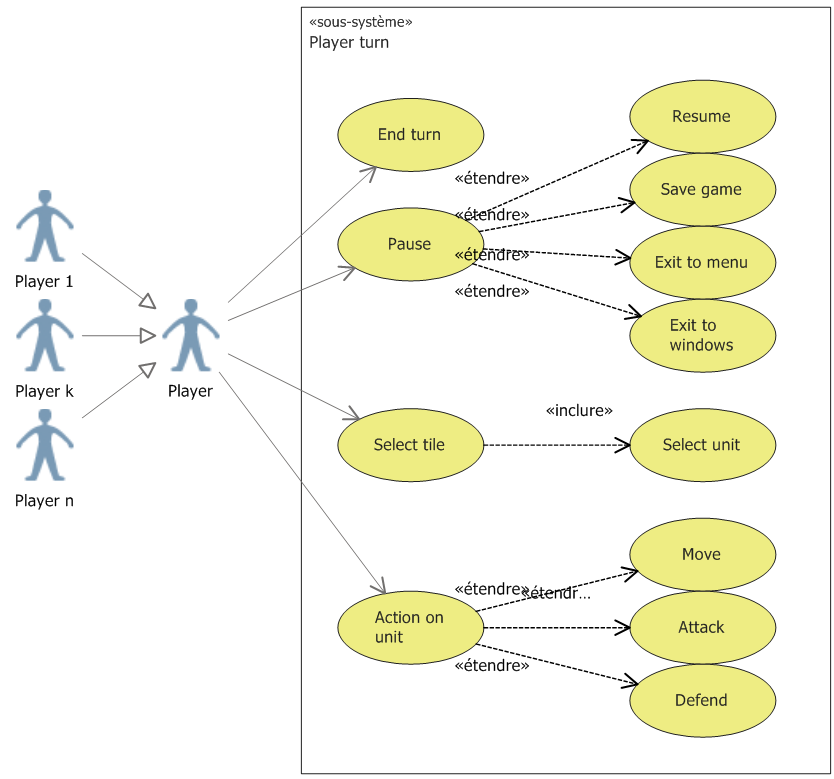
\includegraphics[width=1\textwidth]{figure/cas_util_partie.png}
			\caption{Diagramme de cas d'utilisation - Tour de jeu}
			\label{fig:cas_util_partie}
		\end{figure}
